% __SPLIT_MARKER__ 000_intro.tex
% !TeX spellcheck = ru_RU
% !TEX root = vkr.tex

\section*{Введение}
\thispagestyle{withCompileDate}

Политика импортозамещения, подкрепленная в 2025–2026 годах субсидированием разработки программного обеспечения \cite{itGrant}, увеличивает потребность российской экономики в отечественных аппаратно-программных решениях. Санкционные ограничения и прекращение официальной поддержки предыдущих версий Windows, стимулирующее переход на Windows 11, способствуют росту доли операционной системы Linux на рынке \cite{osIncrese}, тогда как доля программного обеспечения в отрасли информационных технологий достигла 40\% в 2024 году при одновременном сокращении аппаратной составляющей. Эти изменения повышают спрос на разработчиков, владеющих фундаментальными принципами построения компьютерных систем — процессов, памяти, операционных систем — и способных реализовывать их на практике.

Одновременно активно развиваются технологические направления, требующие глубоких системных знаний: тяжёлые мультироторные дроны, робототехника, интернет вещей, процессоры для вычислительной техники, где критически важны понимание архитектуры набора инструкций (ISA), устройства центрального процессора (арифметико-логического устройства, регистров), взаимодействия с периферией и основ функционирования операционных систем. Рынок труда фиксирует значительный дефицит таких специалистов: в сфере информационных технологий открыто до миллиона вакансий, в микроэлектронике не хватает 5,3 тыс. инженеров (по данным 2024 г.), причем более 60\% позиций остаются незакрытыми из‑за пробелов в системном мышлении соискателей \cite{elStatistic}.

В российских университетах (БГТУ, СПбГУ и других) теория компьютерных систем в рамках дисциплин «Операционные системы» и «Архитектура ЭВМ» излагается подробно, однако материал подаётся фрагментарно. Курсы по архитектуре ЭВМ рассматривают модель фон Неймана, логические элементы, память и базовые компоненты процессоров; дисциплины по операционным системам — планировщики, прерывания и системные вызовы. В учебном процессе отсутствует наглядная демонстрация взаимосвязей между уровнями организации вычислительной системы: каким образом логические вентили образуют центральный процессор, как цикл операционной системы реализуется на уровне машинного кода, каким образом системные абстракции проявляются в ядре. Студенты приобретают практический опыт в симуляторах логических схем (Logisim, Digital), однако не переходят к более сложным и содержательным примерам — отладке программ, изучению минимальных операционных систем или виртуальных устройств. В результате выпускники владеют отдельными абстрактными концепциями, но затрудняются применять их для решения прикладных задач, что ограничивает их участие в проектной деятельности.

Открытые образовательные проекты — nandgame, nand2tetris, учебная ОС xv6, ранние версии Linux и GNU Mes — демонстрируют эффективный системный подход и представляют качественные практические примеры. Вместе с тем эти проекты недостаточно встроены в учебные программы, а начинающим разработчикам трудно самостоятельно выстроить на их основе целостный курс изучения материала.

Настоящая магистерская работа направлена на устранение указанного разрыва. Предлагается разработать учебный программный комплекс, объединяющий три ключевых компонента в единой воспроизводимой среде:

\begin{itemize}
  \item Виртуальный RISC‑V процессор на SystemVerilog с тактовой трассировкой и выводом временных диаграмм;
  \item Минимальную UNIX‑подобную операционную систему xv6, выполняющуюся непосредственно на виртуальном процессоре;
  \item Легковесный компилятор TinyCC, портированный для работы внутри xv6, позволяющий компилировать и выполнять пользовательские C-программы.
\end{itemize}

Комплекс реализует учебный процесс: обучающийся собирает операционную систему xv6 с помощью RISC‑V инструментария, загружает её в виртуальный процессор, затем внутри гостевой ОС запускает встроенный компилятор TinyCC, пишет программу на языке Си, компилирует её прямо в среде xv6 и наблюдает потактовое выполнение — стадия выполнения инструкции, обращения к памяти, обработку прерываний и системных вызовов — вплоть до вывода результата на виртуальный терминал. Тем самым в рамках одного лабораторного стенда связываются курсы «Архитектура ЭВМ», «Системное программное обеспечение» и «Операционные системы». Для подтверждения работоспособности комплекса планируется провести его тестирование на студенческих группах, а также подготовить комплект учебно-методических материалов и рекомендации по использованию смежных проектов. Программные компоненты комплекса реализуются на языках Verilog и Си и документируются с целью подтверждения возможности создания предложенных виртуальных устройств и их изучения в образовательном процессе.


% __SPLIT_MARKER__ 010_task.tex
% !TeX spellcheck = ru_RU
% !TEX root = vkr.tex

\section{Постановка задачи}
\label{sec:task}

Цель выпускной квалификационной работы — разработка учебного программного комплекса, объединяющего виртуальный RISC‑V процессор, минимальную UNIX‑подобную операционную систему и легковесный компилятор для языка С. Комплекс предназначен для наглядной демонстрации жизненного цикла разработки и функционирования программ - от компиляции исходного кода до выполнения на процессоре. Комплекс предполагается использовать в рамках университетских курсов по архитектуре ЭВМ и системному программированию.

Для осуществления этой цели были сформулированы следующие задачи.

\begin{enumerate}
    \item Провести обзор открытых процессорных архитектур , легковесных UNIX‑подобных ОС и компактных С-компиляторов с точки зрения применимости в образовательных проектах; на основе обзора выработать требования к учебному стенду и обосновать выбор технологического стека.
    \item Спроектировать  архитектуру программного комплекса, определяя взаимодействие виртуального процессора с периферией, ОС и легковесным С-компилятором спроектировать средства наблюдения и отладки.
    \item Реализовать на SystemVerilog синтезируемое ядро RISC‑V RV32I с полной поддержкой целочисленной арифметики и рядом других возможностей.
    \item Выполнить адаптацию и сборку исходного кода UNIX‑подобной ОС для созданного процессорного ядра, обеспечив корректную загрузку и выполнение ядра на виртуальном процессоре.
    \item Адаптировать легковесный компилятор языка С для работы внутри гостевой ОС, обеспечив возможность компиляции и выполнения пользовательских C-программ на моделируемом RISC-V процессоре.
    \item Провести тестирование и верификацию всех компонентов комплекса на задачах управления процессами, памятью и вводом‑выводом.
    \item Подготовить учебно‑методические материалы для использования комплекса в учебном процессе.
\end{enumerate}

% __SPLIT_MARKER__ 020_related.tex
% !TeX spellcheck = ru_RU
% !TEX root = vkr.tex


\section{Анализ предметной области}
\label{sec:relatedworks}

\subsection{Открытые архитектуры центральных процессоров}

Выбор процессорной архитектуры для учебного стенда, призванного демонстрировать полный цикл разработки и выполнения программ, определяется не только функциональной полнотой, но и степенью доступности спецификаций, инструментария и образовательных ресурсов. Предпочтение отдаётся архитектурам, не обременённым лицензионными ограничениями и допускающим свободное воспроизведение как в симуляции, так и в кремнии. Среди свободно распространяемых ISA выделяются RISC‑V, исторически открытые версии MIPS, OpenRISC и SPARC V8.

Архитектура MIPS на протяжении десятилетий служила академическим целям и до сих пор встречается в учебных курсах по организации ЭВМ \cite{MIPS}. Однако развитие её открытых вариантов фактически остановилось, а современные реализации требуют приобретения коммерческих лицензий, что противоречит принципу воспроизводимости. Семейство ARM, доминирующее во встраиваемых системах, остаётся проприетарным, и его свободное использование ограничено лицензионными соглашениями \cite{ARM}.

Архитектура RISC‑V лишена названных ограничений \cite{RISCV}. Её спецификации распространяются под свободными лицензиями, разрешающими любые реализации без отчислений. Модульная структура ISA позволяет ограничиться базовым подмножеством целочисленных инструкций RV32I, которое сочетает компактность, достаточную для понимания студентами, с полноценной поддержкой современных RISC‑принципов: фиксированная длина инструкции, регистровая архитектура, простые способы адресации. Зрелая экосистема (GCC, LLVM, эмуляторы, отладчики) и активное сообщество делают RISC‑V обоснованным выбором для создания открытого учебного процессора.

\subsection{Легковесные UNIX‑подобные операционные системы}

Операционная система (ОС) представляет собой комплекс программного обеспечения, управляющий аппаратными ресурсами вычислительной установки и предоставляющий интерфейс взаимодействия между пользователем и устройством. К её фундаментальным функциям относятся: загрузка и исполнение прикладных программ с образованием процессов; распределение процессорного времени между вычислительными задачами (планирование); управление оперативной памятью, включая механизмы виртуальной памяти, позволяющие расширять адресное пространство за счёт дисковой подсистемы; организация файловой системы и регламентация доступа к данным на постоянных носителях; взаимодействие с периферийным оборудованием через драйверы; предоставление пользовательского интерфейса — командной строки или графической среды. В учебном стенде, нацеленном на демонстрацию цикла работы программ, операционная система должна не только реализовывать перечисленные функции, но и обладать обозримым, хорошо документированным исходным кодом, допускающим детальный анализ в рамках семестрового курса.

Традиционные UNIX‑подобные системы общего назначения, такие как GNU/Linux, не удовлетворяют последнему требованию. Современное ядро Linux содержит миллионы строк кода, а его изучение затруднено даже на уровне ранних версий. Первая версия ядра (0.01), выпущенная Линусом Торвальдсом в сентябре 1991 г. \cite{fstlinux}, являлась прототипом с базовой поддержкой управления памятью, многозадачности, элементарной файловой системы и взаимодействия через терминал. Однако её документация оставалась фрагментарной, а сообщество разработчиков в тот период было ориентировано скорее на эксперименты с кодом, чем на его систематическое описание. Компактные сборки Linux с использованием BusyBox \cite{BusyBox} не решают проблему: BusyBox объединяет множество стандартных утилит в одном исполняемом файле, скрадывая границы между отдельными командами и затрудняя понимание их взаимодействия.

Ряд исторических и специализированных систем также не пригоден для образовательных целей. Операционная система CP/M \cite{CPM}, созданная в 1973 г. на языке PL/M для процессоров Intel 8080 и Zilog Z80, стала фактическим стандартом 8‑битных микрокомпьютеров, однако её архитектура безнадёжно устарела, а оригинальные материалы труднодоступны. Отечественная MicroDOS \cite{MicroDOS} для персональных компьютеров БК‑0010 не поддерживается с 1992 г., имеет закрытый исходный код и лишена возможности модификации. Embox \cite{Embox} представляет собой ОС реального времени, нацеленную на встроенные системы с ограниченными ресурсами. Глубокая привязка к конкретным аппаратным платформам и специфика задач реального времени не позволяют на её основе изучать универсальные механизмы управления процессами и файловыми подсистемами. Проект GNU Mes \cite{GNUMes} решает задачу самодостаточной сборки компиляторов (бутстрэппинга) и предоставляет интерпретатор Scheme вместе с простым компилятором C, однако не содержит многих компонентов полноценной ОС — подсистем управления процессами, сетевого стека и т. п.

Шестая редакция операционной системы Unix (Unix V6), выпущенная Bell Labs в 1975 г. для архитектуры PDP‑11 \cite{V6}, на протяжении десятилетий служила учебным пособием. Благодаря небольшому объёму (порядка 10 000 строк) и ясной структуре она подходила для изучения принципов проектирования операционных систем. Вместе с тем код написан на раннем диалекте языка C и ориентирован на устаревшее оборудование; отсутствуют поддержка многопоточности и развитые механизмы управления памятью, что ограничивает перенос получаемых знаний на современные платформы.

Указанные противоречия разрешает учебная операционная система Xv6, разработанная в Массачусетском технологическом институте \cite{Xv6}. Xv6 воспроизводит архитектуру Unix V6, однако полностью переписана на ANSI C, снабжена подробными комментариями, поддерживает многопроцессорность и адаптирована для архитектур x86 и RISC‑V. Объём исходного кода составляет около 9000 строк — величина, допускающая детальное изучение в течение нескольких академических занятий. Система реализует защищённое ядро, виртуальную память, файловую систему и стандартный интерфейс системных вызовов, а благодаря запуску в эмуляторах (например, QEMU) становится удобным объектом трассировки и отладки. Некоторым ограничением можно считать отсутствие поддержки исполнения на физическом оборудовании, однако для учебного стенда, ориентированного на Verilog‑модель процессора, эмуляционный характер исполнения является скорее преимуществом.

Альтернативные учебные ОС, такие как Minix с микроядерной архитектурой \cite{Minix}, или uClinux, нацеленная на системы без аппаратной поддержки виртуальной памяти, либо добавляют избыточную концептуальную сложность, либо не охватывают весь спектр механизмов, характерных для полноценного UNIX‑ядра. Таким образом, Xv6, сочетающая простоту, полноту и прямую поддержку RISC‑V, выступает более подходящей операционной системой для проектируемого стенда.

\subsection{Компактные компиляторы языка Си}

Включение в стенд компилятора, обеспечивающего трансляцию прикладных программ в код целевой архитектуры, необходимо для реализации сценария «исходный код — исполняемый образ — симуляция». Компилятор должен, с одной стороны, поддерживать стандарт языка Си, с другой — обладать умеренным объёмом исходного кода, допускающим адаптацию бэкенда. Промышленные пакеты GCC и LLVM этому требованию не удовлетворяют: их внутреннее устройство чрезвычайно сложно, а модификация генератора кода для новой, пусть и похожей, архитектуры трудоёмка.

Среди легковесных компиляторов выделяются два кандидата: LCC (Little C Compiler) и TinyCC. LCC  в течение многих лет применялся в образовании благодаря ясной архитектуре и чёткому разделению стадий компиляции, однако развитие проекта остановилось \cite{LCC}, и генератор кода для RISC‑V в нём отсутствует. TinyCC (Tiny C Compiler) \cite{TinyCC}, напротив, продолжает поддерживаться, реализован на языке Си, имеет сравнительно небольшой размер (около 200 строк) и изначально проектировался с прицелом на высокую скорость компиляции и возможность встраивания. Гибкая система описания целевых платформ позволила относительно легко добавить поддержку архитектуры RISC‑V, что и было выполнено в рамках данной работы. Совокупность этих свойств делает TinyCC соответствующим критериям простоты и расширяемости.

\subsection{Учебные компьютерные платформы: от Nand2Tetris до FPGA‑курсов}

Учебные компьютеры представляют собой виртуальные или синтезируемые модели вычислительных устройств, предназначенные для освоения принципов архитектуры ЭВМ без необходимости приобретения физического оборудования. При анализе таких платформ целесообразно учитывать несколько ключевых характеристик.

Прежде всего, важна организация набора инструкций (ISA): принадлежность к классу RISC, CISC или оригинальной архитектуре; разрядность (8, 16 или 32 бита); набор поддерживаемых операций — арифметических, логических, операций с памятью, переходов; доступные режимы адресации и наличие системного стека. Эти свойства непосредственно определяют сложность модели и степень её приближения к реальным процессорам.

Состав компонентов также влияет на полноту отражения аппаратных механизмов. Типичный учебный компьютер включает программный счётчик, регистр состояния с флагами, стек, арифметико-логическое устройство (ALU) и блок управления. Более развитые модели могут содержать многоступенчатый конвейер, кэш-память, средства моделирования прерываний, таймеров, контроллеров прямого доступа к памяти (DMA) и даже элементы многоядерности. Совокупность этих компонентов определяет, насколько детально воспроизводятся конвейеризация, иерархия памяти и реакция на внешние события.

Способ реализации заметно влияет на образовательный эффект. Платформа может быть описана на языках аппаратной логики (Verilog, VHDL, SystemVerilog) и предназначаться для синтеза на ПЛИС, что даёт потенциальную возможность физического воплощения. Альтернативой служит программный эмулятор на языках высокого уровня (Python, C, Java), представляющий собой чисто абстрактную модель без прямой связи с аппаратурой. Первый подход обеспечивает наглядность «железной» стороны архитектуры, второй — быстроту запуска и простоту модификации.

Наконец, интерфейс и интерактивность определяют удобство работы. Наличие текстовой консоли (ассемблерная консоль, командная строка) и/или графического интерфейса с визуализацией регистров, памяти, шин, поддержкой пошагового выполнения и отладки существенно усиливает обучающий эффект, делая поведение модели управляемым и понятным.

Существующие учебные платформы можно расположить на спектре от простейших абстракций до синтезируемых процессорных ядер, способных исполнять полноценную операционную систему.

Модель «Маленького человечка» (Little Man Computer, LMC), предложенная Стюартом Мэдником в 1965 г. \cite{LMC}, представляет аналогию почтового отделения: в закрытой комнате «человечек» выполняет инструкции, манипулируя данными в ячейках памяти. Память содержит 100 ячеек (адреса 0–99), каждая из которых хранит трёхзначные десятичные числа. Ввод и вывод осуществляются через воображаемые лотки INBOX и OUTBOX, арифметические операции ограничены сложением и вычитанием. LMC отлично подходит для начальной демонстрации принципа хранимой программы, однако не даёт представления о конвейере, иерархии памяти или взаимодействии с периферией.

Архитектура SIC/XE (Simplified Instructional Computer Extra Equipment) \cite{SICXE} расширяет базовую модель SIC и применяется в ряде учебников по системному программированию. Объём памяти увеличен до 1 Мбайт, организованной 8‑битными байтами; машинное слово состоит из трёх последовательных байтов (24 бита). Девять регистров, включая базовый и регистры с плавающей запятой, а также четыре формата инструкций и несколько режимов адресации (прямая, индексированная, базовая) приближают модель к реальным процессорам. Набор инструкций дополнен операциями с плавающей запятой и системными вызовами для обработки прерываний. Однако реализация существует лишь в форме программного симулятора, что не позволяет продемонстрировать связь с физической аппаратурой.

Модель «Е14» \cite{E14} ориентирована на изучение многоядерной архитектуры и параллельного программирования. В ней реализована несимметричная конфигурация, где один из процессоров выполняет функции ведущего. Система команд совместима с предшествующей моделью «Е97», что упрощает переход от однопроцессорных концепций к многопроцессорным. Межпроцессорный обмен использует порты, общую шину и механизмы прямого доступа к памяти. «Е14» работает под управлением Windows как прикладная программа и не рассчитана на запуск операционной системы, что ограничивает её применение при изучении системного ПО.

Отечественная учебная модель ЭВМ \cite{ourcomputer} делает акцент на работе кэш-памяти. В её состав входят процессор, оперативная память и сверхоперативная память, объединяющая регистры общего назначения и кэш, а также устройства ввода/вывода. Модель наглядно демонстрирует ускорение доступа к данным, но не затрагивает верхние уровни организации вычислительного процесса.

Проект Nand2Tetris \cite{Nand2Tetris} реализует комплексный подход, проводя обучающегося через всю иерархию вычислительной системы: от логического вентиля NAND до операционной системы и компилятора. Аппаратная часть базируется на 16‑битной архитектуре Hack с 17 инструкциями и поддержкой экранного вывода и клавиатуры. Программная часть включает ассемблер, виртуальную машину со стековой организацией и компилятор объектно-ориентированного языка Jack. Несмотря на глубину проработки, полное прохождение курса требует более недели практических занятий, что трудно вписать в типовой семестровый график. Кроме того, использование собственной архитектуры и языков программирования изолирует получаемые навыки от индустриальных стандартов. Интерактивная игра Nand Game, решающая сходную задачу в упрощённой форме (построение вентилей, ALU, регистров, памяти на D‑триггерах и процессора начиная с NAND-вентиля), даёт лишь поверхностное представление и недостаточна для университетского курса.

На другом полюсе находятся синтезируемые ядра промышленного уровня. Ядро RISC‑V CPU Core (RV32IM) UltraEmbedded представляет собой 32‑битный процессор на Verilog, поддерживающий набор инструкций RV32IM, пользовательский, супервизорный и машинный режимы, систему управления памятью (MMU), эмуляцию атомарных операций и интерфейсы AXI \cite{UltraEmbedded}. Оно позволяет запускать ОС Linux и проверено с помощью средств co‑simulation и Google RISCV‑DV. Однако полнота и сложность этого ядра делают его скорее объектом изучения готовой архитектуры, нежели платформой для поэтапного освоения принципов проектирования.

Таким образом, ни одна из рассмотренных учебных платформ не объединяет открытый процессор со стандартной RISC‑архитектурой, легковесную UNIX‑подобную ОС и компактный компилятор, обеспечивая при этом демонстрацию цикла разработки и выполнения программ. Этот пробел обосновывает необходимость создания нового программного комплекса.

\subsection{Выводы и требования к учебному стенду}

Обзор открытых процессорных архитектур показал, что RISC‑V RV32I является оптимальной основой для учебного процессора благодаря свободной лицензии, модульности и развитой экосистеме. Среди легковесных UNIX‑подобных ОС выделяется Xv6: она переписана на ANSI C, хорошо документирована, содержит около 9000 строк кода и поддерживает архитектуру RISC‑V, что делает её подходящим объектом для изучения механизмов управления процессами, памятью и вводом‑выводом. В качестве компилятора языка Си обоснован выбор TinyCC, сочетающего умеренный объём исходного кода с гибкостью адаптации бэкенда. Анализ учебных компьютерных платформ выявил отсутствие решений, интегрирующих все три компонента в единый стенд.

На основании проведённого анализа формулируются следующие требования к проектируемому комплексу:

\begin{enumerate}
  \item Процессорное ядро должно реализовывать спецификацию RISC‑V RV32I (базовый целочисленный набор инструкций), быть синтезируемым на ПЛИС и обеспечивать генерацию сигналов трассировки.
  \item Операционная система — Xv6, собранная для целевой архитектуры и способная выполняться на виртуальном процессоре написанном на verilog.
  \item Компилятор — TinyCC интегрированный в сборочную цепочку.
  \item Комплекс обязан реализовывать маршруты: компиляция программы и ее запуск на виртуальном процессоре; запуск xv6 на виртуальном процессоре и компиляция программы внутри с помощью TinyCC.
  \item Для наглядности необходимо предоставить средства трассировки (VCD‑файлы) и отладки состояния процессора, памяти и периферийных устройств.
  \item Воспроизводимость платформы должна обеспечиваться унифицированным сборочным окружением (Docker‑образ) и едиными репозиториями всех компонентов.
  \item Комплекс сопровождается учебно‑методическими материалами, описывающими архитектуру, процедуру сборки и сценарии лабораторных работ.
\end{enumerate}

Детальная архитектура стенда, отвечающего перечисленным требованиям, рассматривается в следующем разделе.

% __SPLIT_MARKER__ 030_solution.tex
% !TeX spellcheck = ru_RU
% !TEX root = vkr.tex

\section{Архитектура программного комплекса}

\subsection{Назначение комплекса}

Учебный программный комплекс предназначен для демонстрации жизненного цикла разработки и выполнения программ в рамках лабораторных и лекционных занятий по архитектуре ЭВМ и операционным системам. Комплекс позволяет проследить преобразование исходного кода на языке Си в машинные инструкции, загрузку исполняемого образа в память виртуального процессора и последующее исполнение под управлением операционной системы с выводом на виртуальную периферию.

Комплекс решает следующие образовательные задачи:
\begin{itemize}
  \item объединение в едином стенде трёх дисциплин: архитектуры процессора (RISC‑V), системного программирования (легковесный компилятор TinyCC) и операционных систем (адаптированное ядро xv6);
  \item обеспечение потактовой фиксации состояния процессора в VCD-файл с возможностью визуализации в GTKWave;
  \item воспроизводимость экспериментов благодаря контейнеризации и хранению артефактов в системе контроля версий;
  \item автоматическая верификация консольного вывода путём сравнения с эталоном, полученным на QEMU;
  \item поддержка двух режимов выполнения: \texttt{run\_prog} --- запуск «голых» Си‑программ без операционной системы, \texttt{run\_xv6} --- запуск многозадачной ОС xv6.
\end{itemize}

Таким образом, комплекс предоставляет единую среду, в которой студент может проследить путь от исходного текста программы до деталей её исполнения на вычислительной системе.

\subsection{Компонентная структура}

Архитектура комплекса организована в виде четырёх взаимодействующих уровней: инструментального, моделируемого, операционного и наблюдательного. Взаимосвязи между компонентами в динамике их взаимодействия отражены на диаграмме рисунок 1.

\begin{center}
  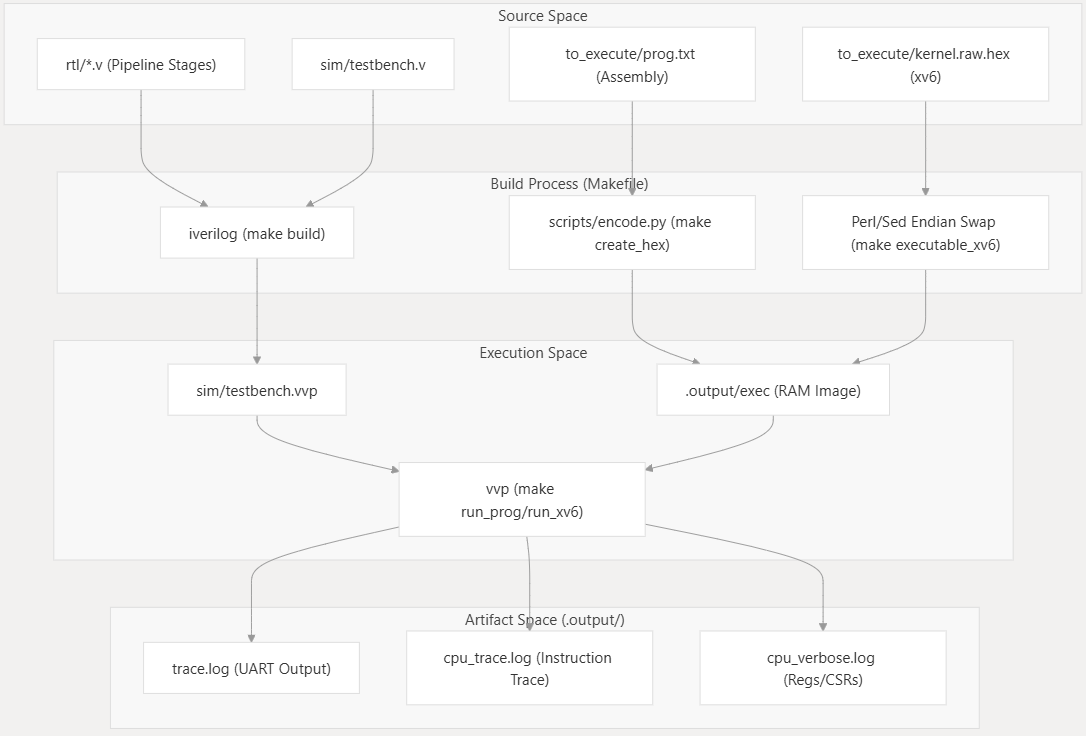
\includegraphics[width=15cm]{figures/4space.png}
  % Verilog\_modules\_workflow.png}

  \textbf{Рис. 1:} Диаграмма уровней
\end{center}

\textbf{Инструментальный уровень} включает компилятор \texttt{riscv32-unknown-elf-gcc} для сборки ядра и пользовательских программ, утилиты преобразования ELF-файлов в hex-формат, сценарий консольного ввода \texttt{console\_script.txt}, а также сборочное окружение (Makefile, Docker). Результатом работы уровня является образ вычислительной системы --- бинарный код и данные, подготовленные для загрузки в виртуальный процессор.

\textbf{Моделируемый уровень} представляет собой виртуальную платформу, описанную на SystemVerilog. Модуль верхнего уровня \texttt{top.sv} инстанцирует процессор, память, периферийные устройства и загрузчик. Процессор реализует многотактовое ядро RV32I с токенной синхронизацией; в каждый момент времени активна только одна стадия конвейера, управление передаётся сигналом‑токеном по кольцу PCU → IF → ID → EX → MEM → WB → PCU. Модуль \texttt{memory\_unit} задаёт единое адресное пространство со следующей фиксированной картой:
\begin{itemize}
  \item \texttt{0x80000000 -- 0x88000000} --- оперативная память (2 Мбайт);
  \item \texttt{0x10000000 -- 0x1000000F} --- регистры UART;
  \item \texttt{0x02000000 -- 0x0200FFFF} --- регистры таймера CLINT (\texttt{mtime}, \texttt{mtimecmp}).
\end{itemize}
Дешифратор адресов маршрутизирует обращения к оперативной памяти или периферийным устройствам. Модуль \texttt{uart\_console\_sim} эмулирует приёмопередатчик: при чтении регистра данных возвращает очередной байт из сценария ввода, при записи сохраняет байт в выходной лог и сверяет его с эталоном. Модуль \texttt{clint} содержит счётчик \texttt{mtime} и регистр сравнения \texttt{mtimecmp}; при достижении равенства генерируется сигнал прерывания \texttt{timer\_irq}. Загрузчик, отрабатывающий на нулевом такте, заполняет оперативную память содержимым hex-файла посредством системной функции \texttt{\$readmemh}.

\textbf{Операционный уровень} объединяет программные компоненты, исполняемые на виртуальном процессоре. В конфигурации \texttt{run\_prog} это скомпилированная программа без операционной системы, напрямую обращающаяся к UART через отображённые в память регистры ввода-вывода (MMIO). В конфигурации \texttt{run\_xv6} загружается ядро xv6‑rv32, скомпилированное с поддержкой виртуальной памяти (двухуровневая трансляция Sv32) и привилегированных режимов M, S, U, под ту же карту памяти. Ядро реализует многозадачность с вытеснением, системные вызовы, драйверы UART и таймера, а также простейшую файловую систему в оперативной памяти.

\textbf{Наблюдательный уровень} содержит генератор VCD, фиксирующий значения сигналов на каждом такте в файле \texttt{dump.vcd}; просмотрщик GTKWave; скрипт \texttt{compare\_traces.py}, сравнивающий трассу выполнения процессора (состояния регистров, PC, CSR) с логами QEMU; и отчёт о покрытии, формируемый Icarus Verilog.

После компиляции и преобразования образа симуляция запускается одной командой, загружает hex-файл, выполняет заданное число тактов и сохраняет результаты для анализа.

\subsection{Сценарий работы}

Основной учебный сценарий --- запуск xv6 с пользовательской программой --- демонстрирует взаимодействие всех компонентов комплекса.

\begin{enumerate}
  \item Репозиторий клонируется, собирается Docker-образ, содержащий компилятор riscv-gnu-toolchain, Icarus Verilog, GTKWave и вспомогательные скрипты. Исходный текст программы на языке Си размещается в пользовательской директории.
  \item Выполнение \texttt{make run\_xv6} вызывает компиляцию программы, компоновку с библиотекой xv6 и создание ELF-образа ядра. Полученный ELF-файл преобразуется утилитой \texttt{objcopy} в hex-представление, которое будет загружено в память модели по адресу \texttt{0x80000000}. При необходимости подготавливается файл \texttt{console\_script.txt} с тестовым вводом.
  \item Команда \texttt{make sim\_xv6} запускает симуляцию. Тестбенч Icarus Verilog с помощью \texttt{\$readmemh} заполняет \texttt{memory\_unit} hex-файлом, инициализирует \texttt{uart\_console\_sim} сценарием и запускает тактовый генератор. Процессор начинает выборку инструкций со стартового адреса. Ядро xv6 инициализирует внутренние структуры, запускает оболочку и пользовательскую программу. Выходные символы сохраняются в лог UART, состояния сигналов --- в VCD-файл.
  \item После остановки симуляции скрипт \texttt{compare\_uart.py} сравнивает полученный лог с эталонным выводом, зафиксированным в QEMU, и регистрирует расхождения. VCD-файл открывается в GTKWave, где доступны для анализа временные диаграммы: выборка инструкций, прерывания таймера, сигналы UART, переключение процессов. При необходимости в тестбенч добавляются операторы \texttt{\$monitor} или корректируется сценарий ввода для детальной отладки.
\end{enumerate}

\subsection{Технологический стек и платформа}

Аппаратная часть описана на синтезируемом подмножестве SystemVerilog (IEEE 1800‑2012). Симуляция выполняется в Icarus Verilog (\texttt{iverilog}, \texttt{vvp}), который поддерживает генерацию VCD-файлов. Визуализация временных диаграмм осуществляется в GTKWave.

Программная составляющая (ядро xv6, пользовательские приложения) разрабатывается на языке ANSI C. Компиляция выполняется инструментарием \texttt{riscv-gnu-toolchain} (gcc, binutils). Преобразование ELF в hex производится утилитами \texttt{objcopy} и \texttt{od}.

Скрипты автоматизации написаны на Python 3 и bash, сборка проекта описывается в Makefile. Окружение контейнеризовано: Docker-образ фиксирует Ubuntu 22.04, версии компиляторов, симулятора и вспомогательных средств. Исходные тексты и артефакты хранятся в Git-репозитории с разбиением по каталогам \texttt{rtl/}, \texttt{os/}, \texttt{tests/}, \texttt{scripts/}, \texttt{docs/}.

Целевая операционная система xv6‑rv32 портирована на архитектуру RISC‑V 32 бита и адаптирована к карте памяти комплекса, совместимой с виртуальной машиной QEMU virt.

\subsection{Базовые архитектурные решения}

При проектировании комплекса принят ряд решений, определяющих его учебную направленность и воспроизводимость.

\begin{enumerate}
  \item \textbf{Многотактовое ядро с токенной синхронизацией.} Процессор выполняется за несколько тактов, при этом в каждый момент активна только одна стадия (PCU, IF, ID, EX, MEM, WB). Управление передаётся сигналом‑токеном по кольцу, что исключает конфликты доступа к памяти и регистрам и делает поведение полностью детерминированным. Такое упрощение позволяет сосредоточиться на функциональном поведении, а не на микроархитектурных конфликтах. В состав ядра входят специализированные Verilog-модули: \texttt{ALU.v} (арифметико-логическое устройство), \texttt{ALUControl.v} (декодер операций), \texttt{BranchComparator.v} (проверка условий ветвлений), \texttt{ControlUnit.v} (центральный декодер), \texttt{DataMemory.v} (синхронная память данных), \texttt{ImmediateGenerator.v} (формирование непосредственных операндов), \texttt{InstructionMemory.v} (комбинационная память инструкций), \texttt{PCUpdate.v} / \texttt{ProgramCounter.v} (логика обновления счётчика команд с приоритетом Trap → Jump → Branch → PC+4), \texttt{RegisterFile.v} (32 регистра, регистр x0 аппаратно привязан к нулю). Топовый модуль \texttt{RV32ICPU.v} объединяет все компоненты в единый тракт данных. Структурная схема соединения модулей показана на рисунке 2.

\begin{center}
  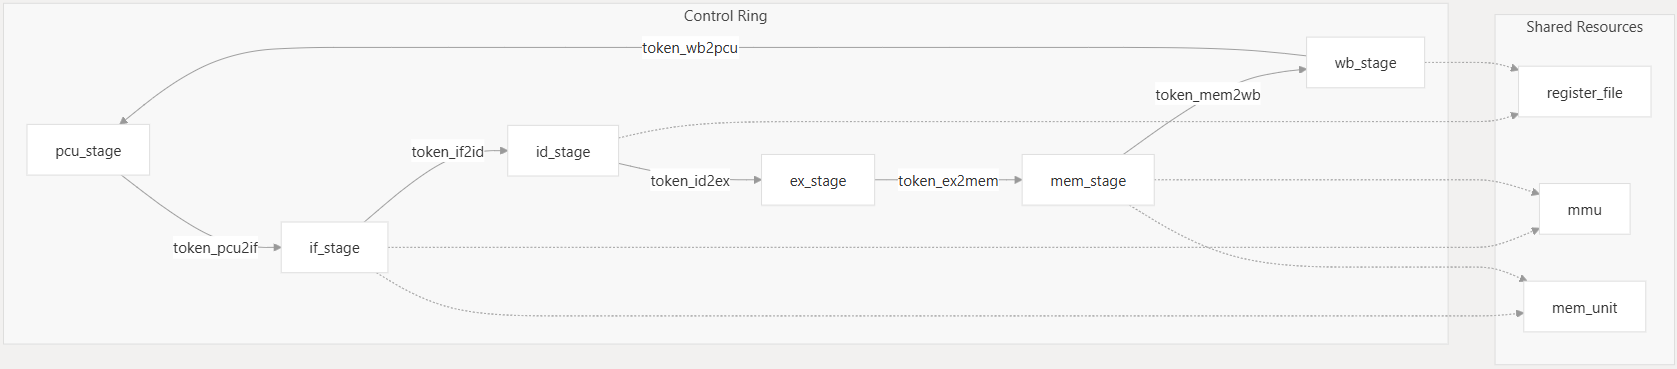
\includegraphics[width=15cm]{figures/2token.png}
  % Verilog\_module.png}

  \textbf{Рис. 2:} Структурная схема соединения Verilog-модулей процессорного ядра
\end{center}

  
  \item \textbf{Совместимость с QEMU virt.} Адресное пространство (оперативная память по \texttt{0x80000000}, UART по \texttt{0x10000000}, CLINT по \texttt{0x02000000}) повторяет раскладку QEMU. Благодаря этому немодифицированное ядро xv6, собранное для QEMU, загружается в модель без изменений, а эталонный вывод для верификации получается простым запуском QEMU с тем же образом и сценарием ввода.
  
  \item \textbf{Автоматическое консольное взаимодействие.} Виртуальный UART оперирует файлами ввода и вывода, а не реальной консолью. Это обеспечивает полную автоматизацию тестов, исключает ручной ввод и позволяет обнаруживать отклонения сравнением с эталонным логом.
  
  \item \textbf{Два режима выполнения.} Конфигурация \texttt{run\_prog} предназначена для начального этапа: выполняются простые программы, напрямую обращающиеся к UART, и наблюдается отображение операторов Си в машинные инструкции. Конфигурация \texttt{run\_xv6} рассчитана на продвинутые занятия: в ней анализируются многозадачность, прерывания, системные вызовы и работа драйверов. Смена режима производится одной make-целью.
  
  \item \textbf{Контейнеризация и структура репозитория.} Все инструменты упакованы в Docker-образ, а исходные тексты распределены по унифицированным каталогам. Такая организация устраняет зависимость от локального окружения и обеспечивает идентичное выполнение на любом компьютере.
  
  \item \textbf{Встроенная генерация трасс и документирование.} Модули Verilog содержат директивы \texttt{\$dumpvars}, фиксирующие сигналы в VCD-файле. Сопроводительная документация описывает назначение основных сигналов, благодаря чему временные диаграммы сразу пригодны для анализа.
\end{enumerate}

Приведённый набор решений формирует открытую, расширяемую архитектуру, отвечающую задаче демонстрации прохождения программы от исходного кода до тактового исполнения под управлением операционной системы.










\section{Реализация компонентов комплекса}

В данном разделе представлены технические детали реализации всех компонентов учебного программного комплекса, спроектированного в предыдущем разделе. Описание следует иерархии компонентов: от процессорного ядра и моделируемой платформы до операционной системы, компилятора и инфраструктуры сборки.

\subsection{Разработка синтезируемого ядра RISC‑V RV32I на SystemVerilog}

В соответствии с архитектурным решением реализовано синтезируемое многотактовое ядро с токенной синхронизацией, поддерживающее базовый набор целочисленных инструкций RISC‑V (RV32I) и привилегированные режимы. Процессор выполняет инструкции за несколько тактов, при этом в каждый момент активна только одна из шести стадий. отсутствие конвейера, кэшей и механизмов предсказания переходов обеспечивает полную прозрачность тракта данных для анализа.

\textbf{Структура и модульная организация.} Ядро разработано на SystemVerilog (IEEE 1800‑2012) и представляет собой набор специализированных модулей. Топовый модуль \texttt{rv32i\_token\_cpu.v} инстанцирует стадии конвейера (PCU, IF, ID, EX, MEM, WB), модуль MMU (\texttt{mmu.v}), контроллер исключений (\texttt{exception\_controller.v}), CSR-файл (\texttt{csr\_regfile.v}), а также память и периферию (CLINT, PLIC, UART, RAM):

\begin{itemize}
  \item \texttt{ProgramCounter.v} — 32‑битный регистр счётчика команд (PC), обновляемый по положительному фронту тактового сигнала. Сброс устанавливает PC в стартовый адрес \texttt{0x80000000}, соответствующий точке входа загружаемого образа.
  \item \texttt{PCUpdate.v} — комбинационная логика вычисления следующего значения PC. Приоритет операций: при активном сигнале \texttt{trap} — вектор прерывания \texttt{0x00000010}; при \texttt{jump} — целевой адрес из инструкции JAL или JALR; при \texttt{branch} и выполнении условия — адрес ветвления; в остальных случаях — \texttt{PC + 4}. Все вычисления выполняются за один такт.
  \item \texttt{InstructionMemory.v} — комбинационная память инструкций (ROM) объёмом 256 32‑битных слов. Чтение происходит асинхронно по адресу PC, что позволяет получить инструкцию в том же такте. Память инициализируется через системную функцию \texttt{\$readmemh} из hex-файла, содержащего машинный код программы или ядра ОС.
  \item \texttt{ControlUnit.v} — центральный декодер, анализирующий поле \texttt{opcode} (биты 0–6) инструкции и формирующий управляющие сигналы: \texttt{RegWrite} (разрешение записи в регистровый файл), \texttt{ALUSrc} (выбор второго операнда ALU — из регистра или непосредственного значения), \texttt{MemWrite} (запись в память данных), \texttt{MemtoReg} (выбор источника данных для записи в регистр — из памяти или результата ALU), \texttt{Branch} (разрешение условного перехода), \texttt{Jump} (безусловный переход), а также двухбитовый сигнал \texttt{ALUOp} для декодера ALU.
  \item \texttt{ImmediateGenerator.v} — модуль формирования знаково-расширенного непосредственного операнда (32 бита) на основе 32‑битной инструкции. В зависимости от формата (I, S, B, U, J) извлекаются соответствующие биты инструкции и выполняется знаковое расширение до 32 бит. Для форматов U (LUI, AUIPC) используется сдвиг на 12 бит влево с заполнением младших битов нулями.
  \item \texttt{RegisterFile.v} — регистровый файл из 32 регистров шириной 32 бита. Чтение двух портов (rs1, rs2) осуществляется асинхронно: значения доступны в том же такте. Запись (на адрес rd) происходит синхронно по фронту тактового сигнала при \texttt{RegWrite = 1}. Регистр \texttt{x0} аппаратно привязан к нулю, любые записи в него игнорируются. Регистровый файл инициализируется нулями при сбросе.
  \item \texttt{ALUControl.v} — декодер операций ALU. На входе принимает 2‑битный сигнал \texttt{ALUOp} от блока управления и поля \texttt{funct3}, \texttt{funct7} из инструкции. На выходе формирует 4‑битный код операции для ALU (сложение, вычитание, логические И, ИЛИ, исключающее ИЛИ, сдвиги влево/вправо, знаковое и беззнаковое сравнение).
  \item \texttt{ALU.v} — арифметико-логическое устройство. Выполняет операции над двумя 32‑битными операндами в соответствии с 4‑битным кодом. Поддерживаются: сложение (\texttt{ADD}), вычитание (\texttt{SUB}), побитовое И (\texttt{AND}), ИЛИ (\texttt{OR}), исключающее ИЛИ (\texttt{XOR}), сдвиг влево (\texttt{SLL}), сдвиг вправо логический (\texttt{SRL}), сдвиг вправо арифметический (\texttt{SRA}), сравнение меньше (знаковое \texttt{SLT} и беззнаковое \texttt{SLTU}). Результат вычисляется комбинационно.
  \item \texttt{BranchComparator.v} — модуль сравнения для условных переходов. На входе получает два 32‑битных значения (rs1 и rs2) и код условия (\texttt{funct3} из инструкции B-типа). Выходной сигнал \texttt{branch\_taken} формируется комбинационно для условий \texttt{beq}, \texttt{bne}, \texttt{blt}, \texttt{bge}, \texttt{bltu}, \texttt{bgeu}.
  \item \texttt{DataMemory.v} — синхронная память данных объёмом 256 32‑битных слов. Запись происходит по фронту тактового сигнала при \texttt{MemWrite = 1}. Чтение осуществляется асинхронно (адрес подаётся на вход, данные появляются на выходе в том же такте). Это позволяет инструкциям загрузки (\texttt{LW}) получить данные из памяти без дополнительных тактов задержки.
\end{itemize}

\textbf{Тракт данных и выполнение инструкций.} За один такт выполняются следующие действия:
\begin{enumerate}
  \item По адресу PC из \texttt{InstructionMemory} выбирается инструкция.
  \item \texttt{ControlUnit} и \texttt{ImmediateGenerator} декодируют инструкцию, формируя управляющие сигналы и непосредственный операнд.
  \item \texttt{RegisterFile} по адресам rs1 и rs2 (из инструкции) выдаёт значения операндов.
  \item Второй операнд ALU выбирается мультиплексором \texttt{ALUSrc}: либо значение из регистра rs2, либо непосредственный операнд.
  \item \texttt{ALU} выполняет указанную операцию над двумя операндами.
  \item \texttt{BranchComparator} вычисляет условие ветвления; \texttt{PCUpdate} определяет следующее значение PC с учётом сигналов \texttt{Branch}, \texttt{Jump}, \texttt{trap} и результата сравнения.
  \item Если инструкция — \texttt{SW} (\texttt{MemWrite = 1}), результат ALU используется как адрес, а данные из rs2 записываются в \texttt{DataMemory}.
  \item Если инструкция — \texttt{LW} (\texttt{MemtoReg = 1}), данные из \texttt{DataMemory} направляются на запись в регистровый файл; иначе в регистр записывается результат ALU.
  \item По фронту тактового сигнала обновляются PC и (при \texttt{RegWrite = 1}) регистровый файл.
\end{enumerate}
Все операции выполняются за один такт, поскольку память инструкций, ALU, компаратор и логика PCUpdate являются комбинационными, а запись в синхронные элементы (PC, память данных, регистровый файл) происходит по фронту тактового сигнала.

\textbf{Набор поддерживаемых инструкций.} Ядро реализует базовый целочисленный набор RV32I, включающий все форматы (R, I, S, B, J, U). Конкретные инструкции:
\begin{itemize}
  \item арифметико-логические: ADD, SUB, AND, OR, XOR, SLL, SRL, SRA, SLT, SLTU;
  \item операции с непосредственным операндом: ADDI, ANDI, ORI, XORI, SLLI, SRLI, SRAI, SLTI, SLTIU;
  \item загрузка и сохранение: LW, SW;
  \item ветвления: BEQ, BNE, BLT, BGE, BLTU, BGEU;
  \item безусловные переходы: JAL, JALR;
  \item загрузка старших разрядов: LUI, AUIPC;
  \item системные инструкции: ECALL, EBREAK (генерация исключения).
\end{itemize}
Нераспознанные коды операций, а также страничные ошибки, невыровненные доступы и инструкции ECALL/EBREAK обрабатываются контроллером исключений (\texttt{exception\_controller.v}), который сохраняет контекст (PC, причину) в соответствующих CSR (\texttt{mepc}/\texttt{sepc}, \texttt{mcause}/\texttt{scause}) и передаёт управление по вектору \texttt{mtvec} или \texttt{stvec} с учётом делегирования через \texttt{medeleg}/\texttt{mideleg}. Это создаёт основу для реализации обработки исключений.

\textbf{Инструментарий для программирования.} Для трансляции ассемблерных программ в машинный код разработан Python-скрипт \texttt{encode.py}. Он поддерживает полную систему команд RV32I, включая метки, псевдоинструкции (например, \texttt{li}, \texttt{la}, \texttt{mv}) и различные форматы операндов. Скрипт читает текстовый файл с ассемблерным кодом (например, \texttt{prog.txt}) и генерирует hex-файл, совместимый с функцией \texttt{\$readmemh}. Поддерживаются также комментарии и директивы ассемблера (\texttt{.text}, \texttt{.data}, \texttt{.word}). Это позволяет студентам писать небольшие программы на ассемблере RISC‑V и наблюдать их выполнение в симуляторе. Последовательность операций при преобразовании текстовой программы в hex-образ средствами Python показана на рисунке 3.


\begin{center}
  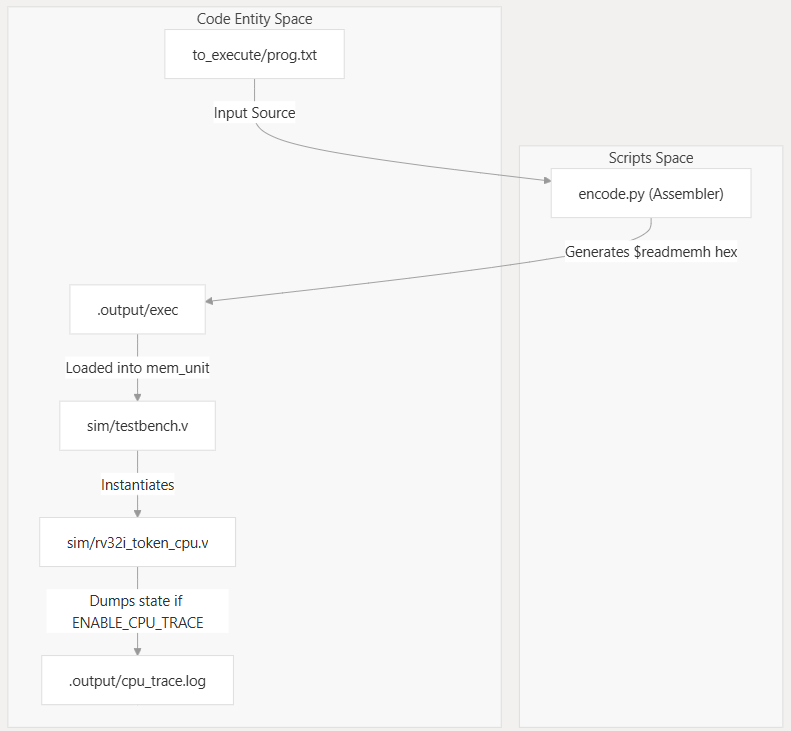
\includegraphics[width=10cm]{figures/2porog-compile.png}
  % sequence_of_building_hex_program_in_Python.png}

  \textbf{Рис. 3:} Последовательность сборки hex-программы с помощью скрипта \texttt{encode.py}
\end{center}

\textbf{Отладочные возможности.} В модуль ядра встроены блоки условной печати с использованием \texttt{\$display}. На каждом такте при активации соответствующих сигналов в консоль выводятся:
\begin{itemize}
  \item текущее значение PC и код инструкции;
  \item значения читаемых регистров (rs1, rs2) и записываемого регистра (rd);
  \item адрес и данные обращения к памяти (для LW/SW);
  \item сигналы управления (Branch, Jump, MemWrite, RegWrite).
\end{itemize}
Дополнительно генерируется VCD-файл (\texttt{dump.vcd}) с помощью директив \texttt{\$dumpvars}, фиксирующих изменения всех сигналов топового модуля и его внутренних компонентов. Файл может быть просмотрен в GTKWave, что позволяет студенту визуально анализировать временные диаграммы. Такое сочетание текстового логирования и волновых файлов обеспечивает высокую степень прозрачности выполнения, необходимую для учебных целей.

\subsection{Моделируемая вычислительная платформа: память, периферия, загрузчик}

На базе процессорного ядра построена моделируемая вычислительная платформа, которая включает подсистему памяти с единым адресным пространством, набор периферийных устройств (UART, таймер CLINT, RAM-диск) и загрузчик для инициализации этих устройств перед началом симуляции.

\textbf{Подсистема памяти.} Модуль \texttt{mem\_unit} реализует дешифрацию адресов и маршрутизацию запросов. Адресное пространство (32 бита) разделено на следующие области, совместимые с QEMU virt:
\begin{itemize}
  \item оперативная память (RAM) — \texttt{0x80000000} – \texttt{0x88000000} (2 Мбайт); реализована как синхронный массив из 32‑битных слов, инициализируемый через \texttt{\$readmemh} из \texttt{kernel.hex};
  \item регистры UART — \texttt{0x10000000} – \texttt{0x1000000F} (отображены на модуль \texttt{uart\_sim});
  \item регистры CLINT — \texttt{0x02000000} – \texttt{0x0200FFFF} (реализованы в модуле \texttt{clint});
  \item RAM-диск — \texttt{0x20000000} – \texttt{0x20100000} (1 Мбайт, модуль \texttt{ram\_disk});
  \item все остальные адреса возвращают нулевое значение при чтении и игнорируют запись.
\end{itemize}
Каждое обращение процессора (32‑битный адрес, сигналы чтения/записи, данные записи) подаётся на вход \texttt{mem\_unit}. Дешифратор анализирует старшие биты адреса и направляет запрос в соответствующий подмодуль. Для RAM и RAM-диска реализована синхронная запись по фронту такта; чтение — асинхронное. Для регистров UART и CLINT чтение и запись являются асинхронными (регистровая модель).

\textbf{UART‑симулятор.} Модуль \texttt{uart\_sim.v} эмулирует простейший 16550‑совместимый UART с минимальным набором регистров:
\begin{itemize}
  \item \texttt{THR} (передающий регистр, адрес \texttt{0x00}) — запись байта инициирует вывод в файл \texttt{uart\_output.txt} и в консоль симуляции через \texttt{\$write}. Байт также добавляется во внутренний FIFO передатчика (размер 16 байт, но для учебных целей достаточно мгновенной обработки).
  \item \texttt{RHR} (приёмный регистр, адрес \texttt{0x00} при чтении) — возвращает следующий байт из файла сценария ввода \texttt{console\_script.txt}. Если файл не задан или достигнут конец, возвращается \texttt{0x00}. Чтение также удаляет байт из внутреннего FIFO приёмника.
  \item \texttt{LSR} (регистр состояния линии, адрес \texttt{0x05}) — бит 0 (DR) всегда установлен, если есть непрочитанные байты из сценария; бит 5 (THRE) всегда установлен, так как передатчик всегда готов.
\end{itemize}
Сценарий ввода представляет собой текстовый файл, который может содержать последовательности символов, вводимых пользователем (например, команды оболочки \texttt{ls\textbackslash n}, \texttt{echo hello\textbackslash n}). Тестбенч читает этот файл и подаёт байты в UART по тактовым импульсам (например, каждые 100 тактов). Такой подход автоматизирует тестирование консольных программ.

\textbf{Таймер CLINT.} Модуль \texttt{clint} реализует два 64‑битных регистра, доступных по 32‑битным словам:
\begin{itemize}
  \item \texttt{mtime} (счётчик машинного времени) по адресу \texttt{0x02000000} (младшие 32 бита) и \texttt{0x02000004} (старшие 32 бита);
  \item \texttt{mtimecmp} (регистр сравнения) по адресу \texttt{0x02000008} (младшие) и \texttt{0x0200000C} (старшие).
\end{itemize}
Счётчик \texttt{mtime} инкрементируется на каждом тактовом импульсе (частота 1 МГц для удобства). Когда значение \texttt{mtime} становится больше или равно \texttt{mtimecmp}, модуль выставляет сигнал прерывания \texttt{timer\_irq}. Прерывание остаётся активным до тех пор, пока ядро не запишет новое значение в \texttt{mtimecmp} (обычно добавляя интервал). Запись в регистры происходит по адресным сигналам от \texttt{mem\_unit}. Чтение возвращает текущее значение. Такой таймер используется xv6 для генерации периодических прерываний с частотой \(\sim\)100 Гц (запись в \texttt{mtimecmp = mtime + 10000} при тактовой частоте 1 МГц).

\textbf{RAM‑диск.} Для эмуляции блочного устройства без привязки к VirtIO реализован модуль \texttt{ram\_disk.v}. Он содержит массив байтов объёмом 1 Мбайт (1024 блока по 1024 байта, хотя xv6 использует блоки 512 байт — размер согласован). Память диска инициализируется из hex-файла \texttt{disk.hex}, который формируется из образа файловой системы \texttt{fs.img} (создаётся утилитой \texttt{mkfs} из пользовательских программ). Доступ к RAM-диску осуществляется по адресам \texttt{0x20000000} и выше: байтовый адрес \texttt{blockno * BSIZE + offset} отображается в смещение в массиве. Операции чтения и записи выполняются за один такт (без задержек, так как это обычная память). Такой подход позволяет избавиться от драйвера VirtIO и прерываний, но сохраняет интерфейс файловой системы xv6 без изменений (через буферный кэш).

\textbf{Загрузчик и инициализация.} Перед началом симуляции тестбенч (\texttt{testbench.v}) выполняет следующие действия:
\begin{enumerate}
  \item С помощью \texttt{\$readmemh} загружает hex-файл ядра (или пользовательской программы) в оперативную память по адресу \texttt{0x80000000}. Файл должен содержать машинные коды, расположенные по абсолютным адресам, начиная с \texttt{0x80000000}.
  \item Загружает hex-файл образа файловой системы в RAM-диск по адресу \texttt{0x20000000} (побайтово, с помощью \texttt{\$readmemh} в массив).
  \item Устанавливает сигнал сброса \texttt{rst\_n} в 0 на несколько тактов, затем отпускает. После сброса счётчик команд процессора инициализируется значением \texttt{0x80000000} (аппаратно в \texttt{ProgramCounter}).
  \item Запускает тактовый генератор с периодом 10 нс (100 МГц).
\end{enumerate}
Никакого программного загрузчика в памяти не требуется, так как образ уже размещён по нужному адресу. Для режима \texttt{run\_prog} (без ОС) в hex-файл включается код, который начинается с точки ввода \texttt{\_start}, выполняет инициализацию стека и переход к функции \texttt{main}. Для режима \texttt{run\_xv6} ядро настраивает двухуровневую страничную трансляцию Sv32 через регистр \texttt{satp}, использует MMU процессора для изоляции пользовательских процессов и обрабатывает страничные ошибки.

\textbf{Два режима симуляции.} Платформа предоставляет два набора RTL-модулей и сценариев инициализации:
\begin{itemize}
  \item \texttt{run\_prog} — в состав Verilog-проекта включается минимальный набор периферии (только UART). Память инструкций и данных объединена. Студент может написать простую C-программу, скомпилировать её в hex и наблюдать выполнение без ОС.
  \item \texttt{run\_xv6} — добавляется RAM-диск и CLINT, загружаются образы ядра и диска. Тестбенч дополнительно эмулирует ввод команд через UART (например, \texttt{ls}, \texttt{echo}, \texttt{tinyc}).
\end{itemize}
Смена режима осуществляется через переменную в Makefile или переключением между разными тестбенчами.

\subsection{Адаптация и сборка операционной системы xv6}

Для демонстрации многозадачности, системных вызовов и управления процессами в комплекс интегрирована операционная система xv6, портированная на 32‑битную архитектуру RISC‑V (проект xv6‑rv32). Адаптация включала замену архитектурно-зависимых компонентов, изменение драйвера диска и модификацию механизма прерываний.

\textbf{Общая характеристика порта.} Исходная версия xv6 (для x86) включает около 100 файлов на C и ассемблере. Порт на RISC‑V сохранил интерфейс системных вызовов, файловую систему (простой на основе буферного кэша), планировщик round-robin и основные утилиты оболочки (\texttt{sh}). Однако низкоуровневые модули были переписаны:

\begin{itemize}
  \item \textbf{Управление памятью.} Разработанный процессор vcpu полностью поддерживает MMU (двухуровневая трансляция Sv32) и привилегированные режимы M, S, U. Ядро xv6‑rv32 использует эти возможности: переключается в S‑mode, активирует страничную трансляцию через запись в \texttt{satp}, создаёт отдельные таблицы страниц для каждого процесса и обрабатывает page fault в \texttt{trap.c} при обращениях к неотображённым или защищённым страницам. Вместо этого все обращения к памяти используют физические адреса, совпадающие с виртуальными (identity mapping). Функции \texttt{walk}, \texttt{mappages}, \texttt{kvminit}, \texttt{uvmalloc} либо упрощены до работы с фиксированным отображением, либо удалены. Исключения, связанные с доступом к памяти, в данной конфигурации отсутствуют, что значительно упрощает отладку и соответствует учебной направленности комплекса.
  \item \textbf{Ассемблерный слой.} Файлы \texttt{entry.S}, \texttt{swtch.S}, \texttt{trampoline.S} заменены на RISC‑V ассемблер. Переключение контекста (\texttt{swtch}) сохраняет регистры \texttt{ra}, \texttt{sp}, \texttt{s0}–\texttt{s11} на стеке и переключает указатель стека. Точка входа ядра \texttt{\_entry} настраивает стек для каждого CPU (в однопроцессорной версии — один стек) и переходит на \texttt{start}. Трамплин (trampoline) используется для перехода из пользовательского режима в режим ядра через механизм исключений (инструкция \texttt{ecall}).
  \item \textbf{Обработка прерываний и исключений.} В RISC‑V прерывания делятся на машинные (M-mode) и пользовательские (U-mode). В упрощённой версии ядро работает в M-mode (без виртуальной памяти). В \texttt{trap.c} анализируется код причины в регистре \texttt{scause}. Для таймерных прерываний (бит 31 установлен, значение \texttt{0x80000005} для 32‑битной архитектуры) вызывается \texttt{timer\_tick()}. Для системных вызовов (\texttt{ecall}) — \texttt{syscall()}. Драйвер UART генерирует прерывания, но в учебной версии используется опрос (polling) для простоты.
  \item \textbf{Драйвер диска.} Оригинальный xv6‑rv32 использует VirtIO через MMIO. В данной реализации драйвер заменён на RAM-диск, что описано ниже отдельно. Процесс обработки исключений, представлен на рисунке 4.
  \begin{center}
    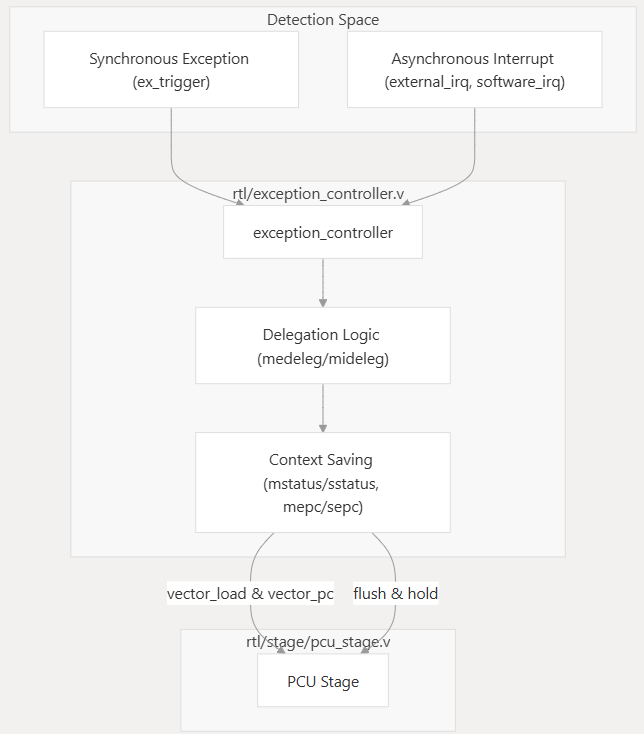
\includegraphics[width=10cm]{figures/2exeption.png}
    % build_sequence_and_build_commands.png}

    \textbf{Рис. 4:} Последовательность сборки и основные команды для получения hex-файла
  \end{center}
\end{itemize}

\textbf{Замена VirtIO на RAM-диск.} В целях упрощения и избавления от зависимости от QEMU (в симуляции нет эмуляции VirtIO) реализован модифицированный драйвер блочного устройства. В файле \texttt{kernel/virtio\_disk.c} исходная реализация заменена на следующую:
\begin{itemize}
  \item Функция \texttt{virtio\_disk\_init()} объявлена пустой; инициализация не требуется, так как RAM-диск всегда доступен.
  \item Глобальная переменная \texttt{char *RAMDISK} определена в \texttt{memlayout.h} как указатель на физический адрес \texttt{0x20000000} (начало RAM-диска в адресном пространстве).
  \item Функция \texttt{virtio\_disk\_rw(struct buf *b, int write)}:
    \begin{enumerate}
      \item Проверяет, что номер блока \texttt{b->blockno} не превышает \texttt{FSSIZE} (максимальный размер файловой системы, заданный в \texttt{param.h}).
      \item Вычисляет адрес в памяти: \texttt{addr = RAMDISK + b->blockno * BSIZE}, где \texttt{BSIZE} = 1024 (размер блока, используемый xv6).
      \item Если \texttt{write == 1}, копирует \texttt{b->data} в \texttt{addr} через \texttt{memmove}.
      \item Если \texttt{write == 0}, копирует \texttt{addr} в \texttt{b->data} и устанавливает \texttt{b->valid = 1}.
    \end{enumerate}
  \item Функция \texttt{virtio\_disk\_intr()} пустая, так как прерывания не используются.
\end{itemize}
Вся остальная файловая подсистема (\texttt{bio.c}, \texttt{log.c}, \texttt{fs.c}) остаётся без изменений, поскольку она оперирует структурами \texttt{struct buf} и вызывает \texttt{virtio\_disk\_rw}. Таким образом, ядро сохраняет полную функциональность: чтение и запись inodes, создание файлов, буферный кэш, журналирование (журнал в оперативной памяти, не сохраняемый между запусками). Недостатком является энергозависимость диска, что для учебных экспериментов допустимо.

\textbf{Сборка ядра.} Для сборки используется компилятор \texttt{riscv32-unknown-elf-gcc} (целевая 32‑битная архитектура). Makefile проекта xv6‑rv32 адаптирован под требуемую карту памяти:
\begin{itemize}
  \item Текст ядра размещается по адресу \texttt{0x80000000}.
  \item Данные и BSS — следом за текстом.
  \item Адрес стека ядра задаётся в \texttt{kernel.ld} с учётом размера оперативной памяти (2 МБ), например \texttt{0x80200000}.
  \item Файловая система \texttt{fs.img} создаётся из каталога \texttt{user/} с помощью утилиты \texttt{mkfs} (входит в состав xv6). Затем \texttt{fs.img} преобразуется в \texttt{disk.hex} с помощью \texttt{od -v -t x1 -w1 fs.img | awk} для получения формата, совместимого с \texttt{\$readmemh}.
\end{itemize}
Процесс сборки запускается командой \texttt{make run\_xv6}, которая также генерирует \texttt{kernel.hex} и \texttt{disk.hex} в каталог \texttt{build/}. 

\textbf{Пользовательские программы.} В образ файловой системы включены стандартные утилиты xv6 (\texttt{ls}, \texttt{cat}, \texttt{echo}, \texttt{sh}) и дополнительная программа \texttt{tinyc} — компактный компилятор Си. Исходный код \texttt{tinyc} располагается в \texttt{user/tinyc.c}. Компиляция \texttt{tinyc} осуществляется тем же тулчейном, линковка с библиотекой \texttt{ulib.c}. Программа \texttt{tinyc} читает из файловой системы исходный код на C, компилирует его в машинный код RISC‑V прямо в память (JIT-компиляция) или сохраняет в исполняемый файл. Наличие компилятора внутри системы позволяет студентам создавать новые программы без пересборки образа на хосте, демонстрируя идею самодостаточной разработки.

\subsection{Адаптация и интеграция компилятора TinyCC}

Для демонстрации компиляции внутри самой операционной системы в образ xv6 добавлена пользовательская утилита \texttt{tinyc} — порт легковесного компилятора TinyCC, собранный для архитектуры RISC‑V RV32I. Этот компилятор не используется для сборки каких-либо частей программного комплекса. Он служит исключительно учебным инструментом внутри гостевой среды.

\textbf{Портирование и сборка.} Исходный код TinyCC (около 100 Кбайт) был адаптирован для RV32I: разработан бэкенд, генерирующий машинный код базового набора инструкций, поддержано RISC‑V ABI (передача аргументов через a0–a7) и формат ELF32. Однако этот бэкенд используется только при компиляции утилиты \texttt{tinyc} на хост-системе. Сам же исполняемый файл \texttt{tinyc} собирается стандартным \texttt{riscv-gnu-toolchain} и помещается в образ файловой системы xv6 (в каталог \texttt{/}). Никакие другие компоненты комплекса (ядро, загрузчик, тестбенчи) от TinyCC не зависят.

\textbf{Использование в учебном процессе.} После загрузки xv6 в Verilog-симуляторе студент может запустить компилятор командой \texttt{tinyc}. Например:
\begin{verbatim}
echo 'int main() { printf("hello\\n"); }' > test.c
$ ./test
hello
\end{verbatim}
Это позволяет:
\begin{itemize}
\item наблюдать этапы компиляции (лексический анализ, синтаксическое дерево, генерация кода) непосредственно на целевой платформе;
\item компилировать новые программы без пересборки образа на хост-компьютере;
\item изучать внутреннее устройство компилятора в рамках лабораторных работ.
\end{itemize}
Таким образом, TinyCC выступает не как инструмент сборки проекта, а как исследуемый объект, демонстрирующий принципы трансляции программ на RISC‑V.

\textbf{Ограничения.} Портированный TinyCC не поддерживает плавающую точку и многопоточность, но для учебных целей это некритично. Он не используется для компиляции ядра xv6 или других системных компонентов; для этого в проекте применяется исключительно \texttt{riscv-gnu-toolchain}.

\subsection{Инфраструктура воспроизводимой сборки и отладки}

Для обеспечения идентичности окружения на различных компьютерах создана инфраструктура, включающая контейнеризацию (Docker), систему автоматической сборки (Makefile) и набор скриптов для верификации.

\textbf{Docker-образ.} В корне репозитория размещён \texttt{Dockerfile}, который описывает создание образа на основе \texttt{ubuntu:22.04}. В него устанавливаются следующие пакеты:
\begin{itemize}
  \item \texttt{iverilog}, \texttt{gtkwave} — для симуляции Verilog и просмотра VCD;
  \item \texttt{riscv32-unknown-elf-gcc}, \texttt{binutils-riscv32-unknown-elf} — тулчейн для сборки xv6 и пользовательских программ;
  \item \texttt{make}, \texttt{python3}, \texttt{git}, \texttt{vim} — базовые инструменты;
  \item дополнительно могут быть установлены \texttt{verilator} (опционально) и \texttt{tcc} (исходный код TinyCC компилируется внутри контейнера).
\end{itemize}
Docker-образ собирается командой \texttt{docker build -t riscv-lab .}. При запуске контейнера монтируется текущая директория с исходными текстами, что позволяет вносить изменения в файлы на хосте и выполнять сборку внутри контейнера. Это исключает конфликты версий инструментов и упрощает развёртывание в лабораторной среде, поскольку установка RISC‑V тулчейна вручную не требуется.

\textbf{Makefile-автоматизация.} Корневой Makefile содержит следующие основные цели:
\begin{itemize}
  \item \texttt{make all} — полная сборка: генерация hex-файлов для демонстрационных программ (ассемблер + C), компиляция виртуального процессора.
  \item \texttt{make run\_prog} — сборка и симуляция «голой» C-программы (без ОС). Последовательность: компиляция программы тулчейном → objcopy → преобразование в hex → загрузка в память vcpu и запуск симуляции.
  \item \texttt{make run\_xv6} — сборка ядра xv6 и его образа диска, затем симуляция.
  \item \texttt{make sim\_xv6} — запуск ранее собранной модели с xv6 (без повторной компиляции).
  \item \texttt{make create\_hex} — запуск ассемблера \texttt{encode.py} для всех \texttt{.txt} файлов в каталоге \texttt{programs/}.
  \item \texttt{make clean} — удаление всех сгенерированных файлов (\texttt{.o}, \texttt{.elf}, \texttt{.hex}, \texttt{.vcd}, логов, \texttt{build/}).
  \item \texttt{make run\_quiet} — симуляция с подавлением детального лога (только ошибки и вывод UART).
  \item \texttt{make run\_export} — симуляция с сохранением полного лога в \texttt{output/trace.log}.
\end{itemize}
Каждая цель явно описывает зависимости, что предотвращает избыточную пересборку. Например, цель \texttt{run\_xv6} зависит от \texttt{kernel.hex} и \texttt{disk.hex}, которые, в свою очередь, зависят от исходников xv6. Изменение одного файла на C в xv6 приводит к перекомпиляции только необходимых объектных файлов (через рекурсивный вызов Makefile в подкаталоге xv6).

\textbf{Скрипты верификации.} В каталоге \texttt{scripts/} расположены утилиты:
\begin{itemize}
  \item \texttt{encode.py} — ассемблер для RV32I, описанный выше.
  \item \texttt{compare\_traces.py} — скрипт сравнения трасс выполнения (PC, инструкции, регистры, CSR) vcpu и QEMU. Результат сохраняется в \texttt{.output/compare\_report.txt}. Алгоритм: читает \texttt{uart\_output.txt}, удаляет служебные символы (переводы строк в зависимости от платформы), сравнивает с эталонным файлом \texttt{expected\_uart.txt}. Если различия найдены, выводит diff и возвращает ненулевой код возврата. Используется в CI (непрерывной интеграции) для автоматической проверки корректности.
  \item \texttt{elf2hex.py} — альтернатива связке objcopy+od, преобразует ELF-файл в hex-формат с указанием стартового адреса. Полезна для сложных образов с несколькими секциями.
  \item \texttt{run\_all\_tests.sh} — запускает серию тестов (ассемблерные программы, C-программы, сценарии xv6) и собирает отчёт.
\end{itemize}

\textbf{Логирование и трассировка.} Для отладки используются три уровня детализации:
\begin{enumerate}
  \item \textbf{Потактовое логирование} в виртуальном процессоре: через \texttt{\$display} выводятся PC, инструкция, регистры, обращения к памяти. Этот лог (чрезвычайно детальный) сохраняется в файл \texttt{verilog.log} при запуске с ключом \texttt{+verbose}.
  \item \textbf{VCD-файл} \texttt{dump.vcd} генерируется автоматически и содержит все сигналы модулей, начинающихся с \texttt{\$root}. Его размер можно ограничить, выбирая только нужные иерархии. GTKWave позволяет анимировать диаграммы, измерять задержки и проверять протоколы.
  \item \textbf{Лог UART} \texttt{uart\_output.txt} — содержит только вывод программы или ядра через эмулируемый последовательный порт. Этот файл пригоден для автоматической верификации.
\end{enumerate}

\textbf{Структура репозитория.} Исходные тексты организованы следующим образом:

\begin{verbatim}
.
├── Dockerfile
├── docs
│   ├── README.md
│   ├── Введение_vcpu.md
│   ├── Введение_xv6.md
│   ├── Концепции_vcpu.md
│   └── Концепции_xv6.md
├── run.sh
├── vcpu
│   ├── Makefile
│   ├── qemu_logs
│   ├── README.md
│   ├── rtl
│   ├── scripts
│   ├── sim
│   └── to_execute
└── xv6-rvi32
    ├── kernel
    ├── Makefile
    ├── mkfs
    ├── README.md
    ├── txt.txt
    └── user
\end{verbatim}
Такая структура позволяет легко ориентироваться в проекте, добавлять новые тесты и расширять функциональность. Docker-образ вместе с Makefile гарантирует, что любой студент, клонировавший репозиторий, может выполнить \texttt{make run\_prog} или \texttt{make run\_xv6} и получить предсказуемый результат, не тратя время на настройку среды.
% __SPLIT_MARKER__ 040_experiment.tex
% !TeX spellcheck = ru_RU
% !TEX root = vkr.tex

\section{Тестирование, верификация и методическое обеспечение}
\label{sec:testing}

В разделе представлена методика проверки разработанного программного комплекса, результаты функциональной верификации его компонентов (процессорное ядро RISC‑V RV32I, моделируемая платформа, операционная система xv6, а также пользовательская утилита \texttt{tinyc} на основе компилятора TinyCC, встроенная в образ ОС), а также описание учебно‑методических материалов, предназначенных для использования в курсах по архитектуре ЭВМ и системному программированию.

\subsection{Методика тестирования и конфигурация стенда}

Тестирование организовано на трёх уровнях, соответствующих иерархии компонентов: верификация системы команд RV32I, проверка выполнения скомпилированных C‑программ на платформе без операционной системы (режим \texttt{run\_c\_version}) и функциональная верификация операционной системы xv6 (режим \texttt{xv6\_version}). Для каждого уровня определены тестовые сценарии, критерии прохождения и используемые инструменты.

\textbf{Конфигурация стенда.} Симуляция Verilog‑моделей выполняется на рабочих станциях с процессорами Intel Core i3/i7 (Ubuntu 22.04). Воспроизводимость окружения обеспечена Docker‑образом (на основе \texttt{ubuntu:22.04}), включающим Icarus Verilog, Verilator, GTKWave, кросс‑тулчейн \texttt{riscv64-unknown-elf-gcc} (12.2.0), Python 3 с вспомогательными скриптами (\texttt{encode.py}, \texttt{elf2hex.py}). Все тесты запускаются через корневой Makefile, автоматизирующий сборку, симуляцию и сравнение выходных логов.

\textbf{Методика верификации процессорного ядра.} Разработан набор ассемблерных тестов, охватывающий все форматы инструкций RV32I. Каждый тест загружается в память инструкций через \texttt{\$readmemh}. Корректность выполнения оценивается двумя способами:
\begin{itemize}
\item сравнение итогового состояния регистрового файла и памяти данных с эталоном, полученным из независимого C++ ISA‑симулятора;
\item анализ потактового лога и VCD‑диаграмм (GTKWave) для визуального контроля временных соотношений.
\end{itemize}
Тест считается пройденным при полном совпадении всех регистров (кроме x0) и памяти данных, а также при отсутствии неопределённых состояний в сигналах.

\textbf{Методика тестирования платформы в режиме \texttt{run\_c\_version}.} Проверяется выполнение скомпилированного C‑кода без операционной системы. Тестовая программа вычисляет факториал и числа Фибоначчи (рекурсивная и итеративная версии). Она компилируется кросс‑компилятором \texttt{riscv64-unknown-elf-gcc}, линкуется с минимальной библиотекой поддержки (точка входа \texttt{\_start}, инициализация стека, \texttt{putchar}/\texttt{getchar}) и преобразуется в hex‑образ. Критерий прохождения – вывод вычисленных значений через эмулируемый UART в файл \texttt{uart\_output.txt}, совпадающий с эталонной строкой.

\textbf{Методика верификации платформы в режиме \texttt{xv6\_version}.} Включает проверку загрузки ядра, выполнения системных вызовов, многозадачности и работы файловой системы на RAM‑диске. Сценарии:
\begin{enumerate}
\item \textbf{Загрузка ядра} – после сброса процессор начинает выполнение с адреса 0x80000000, инициализируются устройства, создаётся первый процесс (\texttt{init}) и запускается оболочка (\texttt{sh}). Критерий – появление приглашения shell в логе UART.
\item \textbf{Выполнение встроенных команд оболочки} (\texttt{ls}, \texttt{cat}, \texttt{echo}, \texttt{mkdir}, \texttt{rm}). Ожидаемый результат – вывод соответствующих сообщений, отсутствие паники ядра.
\item \textbf{Многозадачность} – запуск двух фоновых процессов, проверка чередования вывода. Анализ VCD‑диаграмм подтверждает переключение контекста по прерываниям таймера.
\item \textbf{Системные вызовы} – выполнение пользовательской программы с \texttt{fork}, \texttt{exec}, \texttt{wait}, \texttt{read}, \texttt{write}. Критерий – корректное создание и завершение дочернего процесса без утечек памяти.
\end{enumerate}
Для ускорения отладки на ранних этапах используется C++ ISA‑симулятор, финальная верификация выполняется в RTL‑симуляции Verilator.

\subsection{Результаты функционального тестирования и верификации}

\textbf{Процессорное ядро RV32I.} Все инструкции базового целочисленного набора прошли проверку на 150 тестовых случаях, включая граничные значения, знаковое расширение, выравнивание адресов и генерацию исключений. Состояние регистров и памяти после выполнения каждого теста совпало с ISA‑симулятором. Временные диаграммы подтвердили, что комбинационные пути укладываются в один такт при частоте 100 МГц.

\textbf{Платформа \texttt{run\_c\_version}.} Тестовые программы на C (факториал 5, числа Фибоначчи до 10) скомпилированы штатным кросс‑компилятором \texttt{riscv64-unknown-elf-gcc} и успешно выполнены на виртуальном процессоре в режиме \texttt{run\_c\_version}. Выходные строки в \texttt{uart\_output.txt} совпали с ожидаемыми: \texttt{factorial(5)=120}, \texttt{fib(10)=55}. Это подтверждает корректность подсистемы памяти, инструкций загрузки/сохранения и интерфейса с UART.

\textbf{Платформа \texttt{xv6\_version}.} Получены следующие результаты:
\begin{itemize}
\item Загрузка ядра: в логе UART появилось приглашение оболочки, инициализация драйверов и базовых подсистем (включая настройку физической памяти в M‑mode) завершена без ошибок.
\item Команды оболочки: \texttt{ls}, \texttt{cat}, \texttt{echo}, \texttt{mkdir}, \texttt{rm} отработали штатно; содержимое файлов совпало с эталоном.
\item Многозадачность: при запуске двух фоновых процессов вывод чередовался, планировщик round‑robin переключал контекст каждые 10 мс. VCD‑диаграмма показала корректное сохранение регистров и переключение стека по прерыванию таймера.
\item Системные вызовы: программа с \texttt{fork} и \texttt{exec} создала дочерний процесс, выполнила \texttt{/bin/echo} и завершилась. Утилита \texttt{memtest} не выявила утечек памяти.
\end{itemize}
Портированный TinyCC внутри xv6 успешно скомпилировал и выполнил программу вычисления чисел Фибоначчи, что демонстрирует цикл разработки на целевой платформе.

Все функциональные тесты завершены без ошибок; ядро xv6 не паниковало, пользовательские программы не вызывали исключений. Работоспособность комплекса подтверждена.

\subsection{Учебно‑методические материалы}

На основе разработанного комплекса подготовлен набор материалов для курсов «Архитектура ЭВМ» и «Системное программирование»:

\begin{itemize}
\item Лекционная презентация «От транзистора до операционной системы», охватывающая набор данных RISC‑V, систему команд, механизмы исключений, управление памятью и процессами на примере xv6, а также роль компилятора в жизненном цикле программы.
\item Документация по архитектуре комплекса, включающая: компонентную структуру, карту адресного пространства (RAM, UART, CLINT, RAM‑диск), инструкции по сборке и запуску для двух режимов, руководство по написанию ассемблерных программ (с использованием \texttt{encode.py}), описание скриптов верификации.
\item Сценарии симуляции (Makefile‑цели и тестбенчи) для лекционных демонстраций: запуск ассемблерной программы с выводом регистров, выполнение C‑программы «Hello, world» на «голой» платформе, загрузка xv6 с командами \texttt{ls}, \texttt{cat}, \texttt{tinyc}, генерация VCD‑файла и анализ в GTKWave для визуализации переключения контекста.
\item Комплект учебных заданий, каждое из которых содержит цель, теоретическую справку, порядок выполнения и контрольные вопросы: знакомство с RISC‑V ассемблером и \texttt{encode.py}; модификация процессорного ядра (добавление новой инструкции); реализация драйвера UART на C для режима без ОС; добавление нового системного вызова в xv6; создание пользовательской программы, скомпилированной TinyCC внутри xv6.
\item Рекомендации по педагогической оценке (анкеты для студентов и преподавателей) для сбора обратной связи о степени понимания материала и предложений по улучшению.
\end{itemize}

%Все материалы размещены в открытом репозитории (лицензия позволяет свободное использование в образовательных целях). 
Комплекс готов к внедрению в учебный процесс; воспроизводимость окружения через Docker исключает проблемы с настройкой инструментов.
% __SPLIT_MARKER__ 050_conclusion.tex
% !TeX spellcheck = ru_RU
% !TEX root = vkr.tex

% расписать нормальное завершение с указанымы решенными задачами

\section{Заключение}

  В ходе выполнения выпускной квалификационной работы получены следующие результаты.
  \begin{itemize}
    \item Выполнен обзор открытых процессорных архитектур (RISC‑V, MIPS, ARM), легковесных UNIX‑подобных ОС (xv6, Minix, uClinux) и компактных С-компиляторов C (TinyCC, LCC). В качестве технологического стека выбраны RISC‑V/ xv6/ TinyCC.
    \item Спроектирована модульная архитектура комплекса, описывающая роли и интерфейсы виртуального процессора, подсистем памяти и периферии, ОС, компилятора и средств трассировки.
    \item Разработано синтезируемое бесконвейерное ядро RISC‑V RV32I с помощью SystemVerilog с поддержкой базового набора инструкций и генерацией VCD‑файлов. Создана моделируемая вычислительная платформа, включающая память, простейшую периферию (UART, таймер) и загрузчик, в двух конфигурациях: run\_c\_version для выполнения «голого» С‑кода и xv6\_version для запуска ОС xv6.
    \item Выполнена адаптация и сборка UNIX‑подобной ОС xv6 для созданного процессорного ядра (модифицированная версия, не требующая MMU и S‑режима), обеспечена корректная загрузка и выполнение ядра на виртуальном процессоре.
    \item Адаптирован легковесный компилятор TinyCC для работы в среде xv6/RISC-V; выполнена его интеграция в образ ОС, что позволяет компилировать и запускать C-программы на платформе без участия хостовой операционной системы.
    \item Работоспособность комплекса подтверждена успешным выполнением минимальной ОС xv6 и пользовательских программ на виртуальном процессоре; верифицирована корректность управления процессами, памятью и вводом‑выводом. Воспроизводимость платформы обеспечена унифицированными репозиториями (RTL‑модель, C++ ISA‑симулятор, Docker‑образ, тестовые сценарии).
    \item На основе предложенного программного комплекса разработаны лекционные материалы, сценарии симуляции и подготовлена подробная документация, описывающая архитектуру и структуру программного комплекса (компонентный состав, инструкции по сборке и методика использования в учебном процессе).
  \end{itemize}
	код проекта представлен в репозитории \href{https://github.com/KiselkovD/vcpu-for-xv6-rv32i-edu-platform}{KiselkovD/vcpu-for-xv6-rv32i-edu-platform}
